\newcommand{\basedir}{../fablab-document/} % Pfad zur Dokumentenvorlage
\documentclass{\basedir/fablab-document}
\usepackage{CJK}

%\setCJKmainfont{SimSun.ttf}
%\setCJKsansfont{SimHei.ttf}
%\setCJKmonofont{SimFang.ttf}

\title{FAU FabLab Reisebericht August 2016}
% \author{Dagobert Duck}

\begin{document}

\begin{figure}[htbp]
	\noindent\makebox[\textwidth]{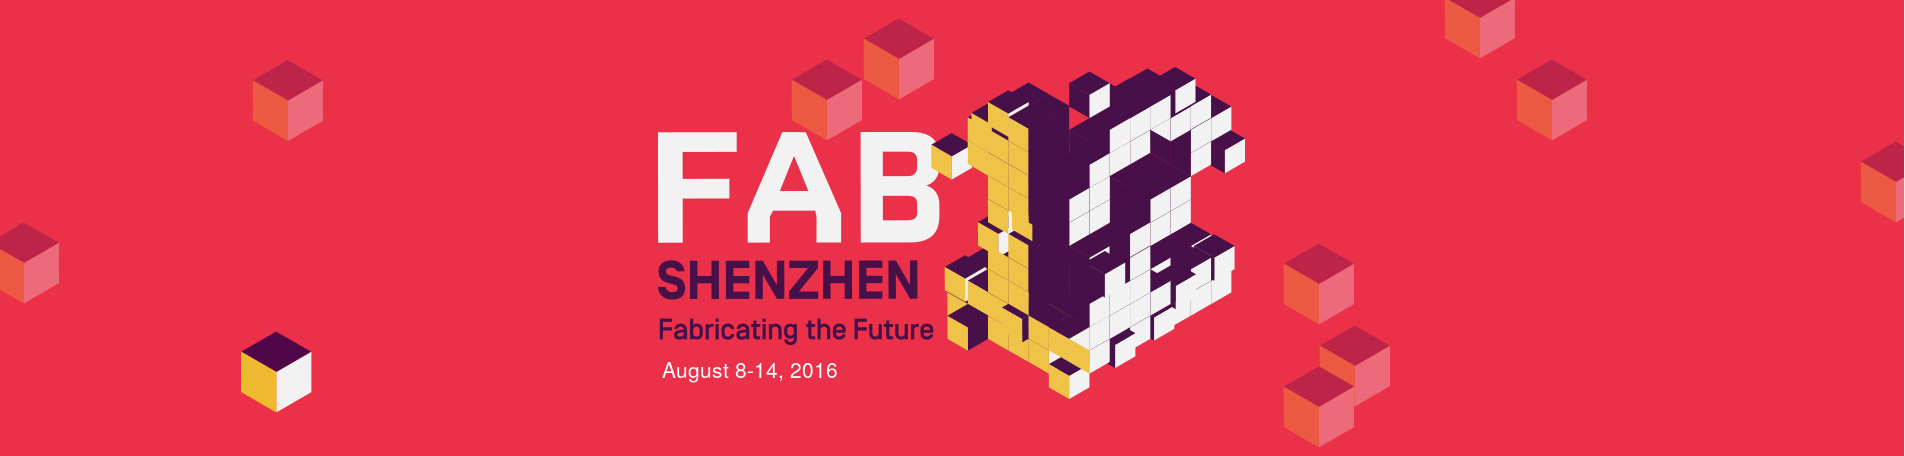
\includegraphics[width=\paperwidth]{img/fab12_banner.png}}
\end{figure}

\section*{}

Vom 8. bis zum 14. August fand in der Mitte Shenzhens in China die Fab12
statt - die zwölfte Auflage der weltweiten FabLab Konferenz. Das
diesjährige Motto war ``Fabricating the Future''. Michael Jäger,
Valentin Olpp, Markus Fritscher und Sebastian Endres waren dank
Studienzuschüssen aus den Departments Maschinenbau und Informatik mit
dabei. Kaum eine andere Stadt wäre besser für eine derartige
Maker-Konferenz geeignet gewesen als Shenzhen: Dort wo ein Großteil der
Elektronik-Bauteile der Welt verkauft und verschickt werden. Ein ganzes
Stadtviertel ist voll mit Elektromärkten, die ein so breites Spektrum
aufweisen, dass jeder Wunsch eines Bastlers in Erfüllung geht. Die junge
Stadt ist in vielen Punkten europäischen Städten vorraus, was perfekt
zum Motto der Konferenz gepasst hat.

Da wir bereits einige Tage früher angereist sind, konnten wir und schon
vorab mit der Stadt etwas vertraut machen. Die eigentliche Konferenz
begann schließlich am Abend des \textbf{9. Augusts} mit der
Registrierung. Bereits hier haben wir viele bekannte Gesichter aus den
vorherigen Jahren getroffen und konnten uns über Neuerungen in unseren
FabLabs austauschen.

Am \textbf{Dienstag} Morgen ging es dann mit Vorträgen und einem Talk
los, nach dem Mittagessen kam dann der aktive Teil für uns. Wir wurden
in mehreren Workshops und sogenannten ``Foo-Sessions'', die eine Art
spontanen Workshop darstellen, gefordert. Unter anderem haben wir im
Shenzhen Open Inovation Lab am Workshop zum Färben von Stoffen mithilfe
von Bakterien teilgenommen, eine geneuere Beschreibung ist unten zu
finden. Am Abend war eine Poolparty geplant, die aber aufgrund eines
Taifuns buchstäblich ins Wasser gefallen ist und durch eine ``Party'' im
Konferenzsaal ersetzt wurde.

\begin{figure}[htbp]
	\noindent\makebox[\textwidth]{
		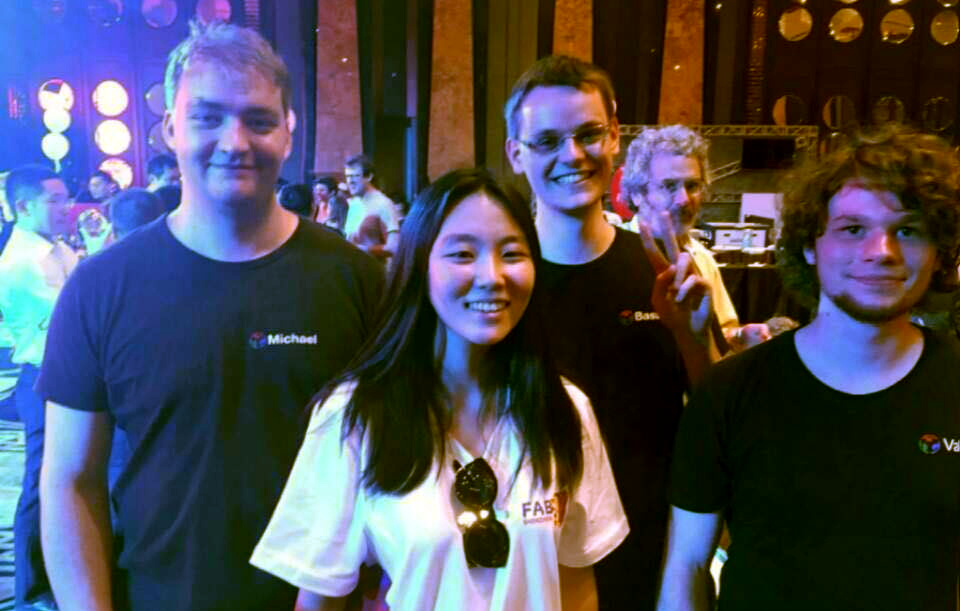
\includegraphics[width=\paperwidth]{img/photobomb_neil.jpg}
	}
	\caption{``Poolparty'' im Sheraton inkl. Photobomb von Neil Gershenfeld}
	\label{photobomb-neil}
\end{figure}

Am \textbf{Mittwoch und Donnerstag} war der Ablauf ähnlich, morgens
stellten sich zuerst lokale Unternehmen und Sponsoren vor, anschließend
gab es jeweils einen Talk. Darunter war eine sehr interssante
Projektvorstellung von \href{http://fabmodules.org/}{FabModules}, eine
Doktorarbeit am MIT. Dabei hat man versucht, das Zusammenspiel der
einzelnen Komponenten eines FabLabs so einfach wie möglich zu gestalten.
Das Ergebnis sind digitale Pipelines, bei denen man den Weg der
Eingabedaten bis hin zur Maschine am Computer zusammenstellen kann. Wenn
es gut funktioniert ist dies auch für unser FabLab interessant.

Neben diversen Workshops gab es auch einige Field Trips zu lokalen
Unternehmen, unter anderem zu \href{https://www.seeedstudio.com/}{SEEED
Studio}, einem Unternehmen, dass sich auf die Entwicklung und Produktion
von Platinen spezialisiert hat. Von Einzelstücken über Kleinserien bis
hin zu Großsserien kann hier alles entwickelt und gefertig werden. Mehr
dazu unter Workshops.

Am \textbf{Mittwoch} Abend wurden wir zum einem Dinner bei 
\href{https://www.3nod.com.cn/en/}{3nod} eingeladen. Nach einer
Führung durch das äußerst fortschrittliche Startup-Büro-Gebäude stellte
der CEO der Firma die Entwicklung und Aufgaben der Firma vor.
Schließlich sicherte er im Namen des gesamten Unternehmes die
Unterstützung der \href{https://fabfoundation.org/}{FabFoundation} zu.
Die pompöse Aufmachung hat uns alle sehr überrascht.

Das Programm am \textbf{Donnerstag} Abend beinhaltete einen Besuch des
\href{https://hax.co/about/}{HAX coworking spaces}. Es ist direkt neben
dem großen \href{https://en.wikipedia.org/wiki/SEG_Plaza}{SEG Platzes},
wo ein Großteil der Elektronikmärkte in Shenzhen angesiedelt sind. Also
der idealste Ort für Bastler. Das Konzept des Hax ist es, ähnlich wie
bei 3nod, die Möglichkeit zu bieten, aus Ideen Startups zu gründen.

\section*{Symposium}

Ab Freitag verlagerte sich der Ort des Geschehens vom Sheraton Hotel zum
Convention Center. Dort gab es neben weiteren Vorträgen eine Ausstellung
von Maschinen, die man häufig in FabLabs vorfindet, aber auch von
neuartigen Geräten.

\begin{figure}[htbp]
	\noindent\makebox[\textwidth]{
		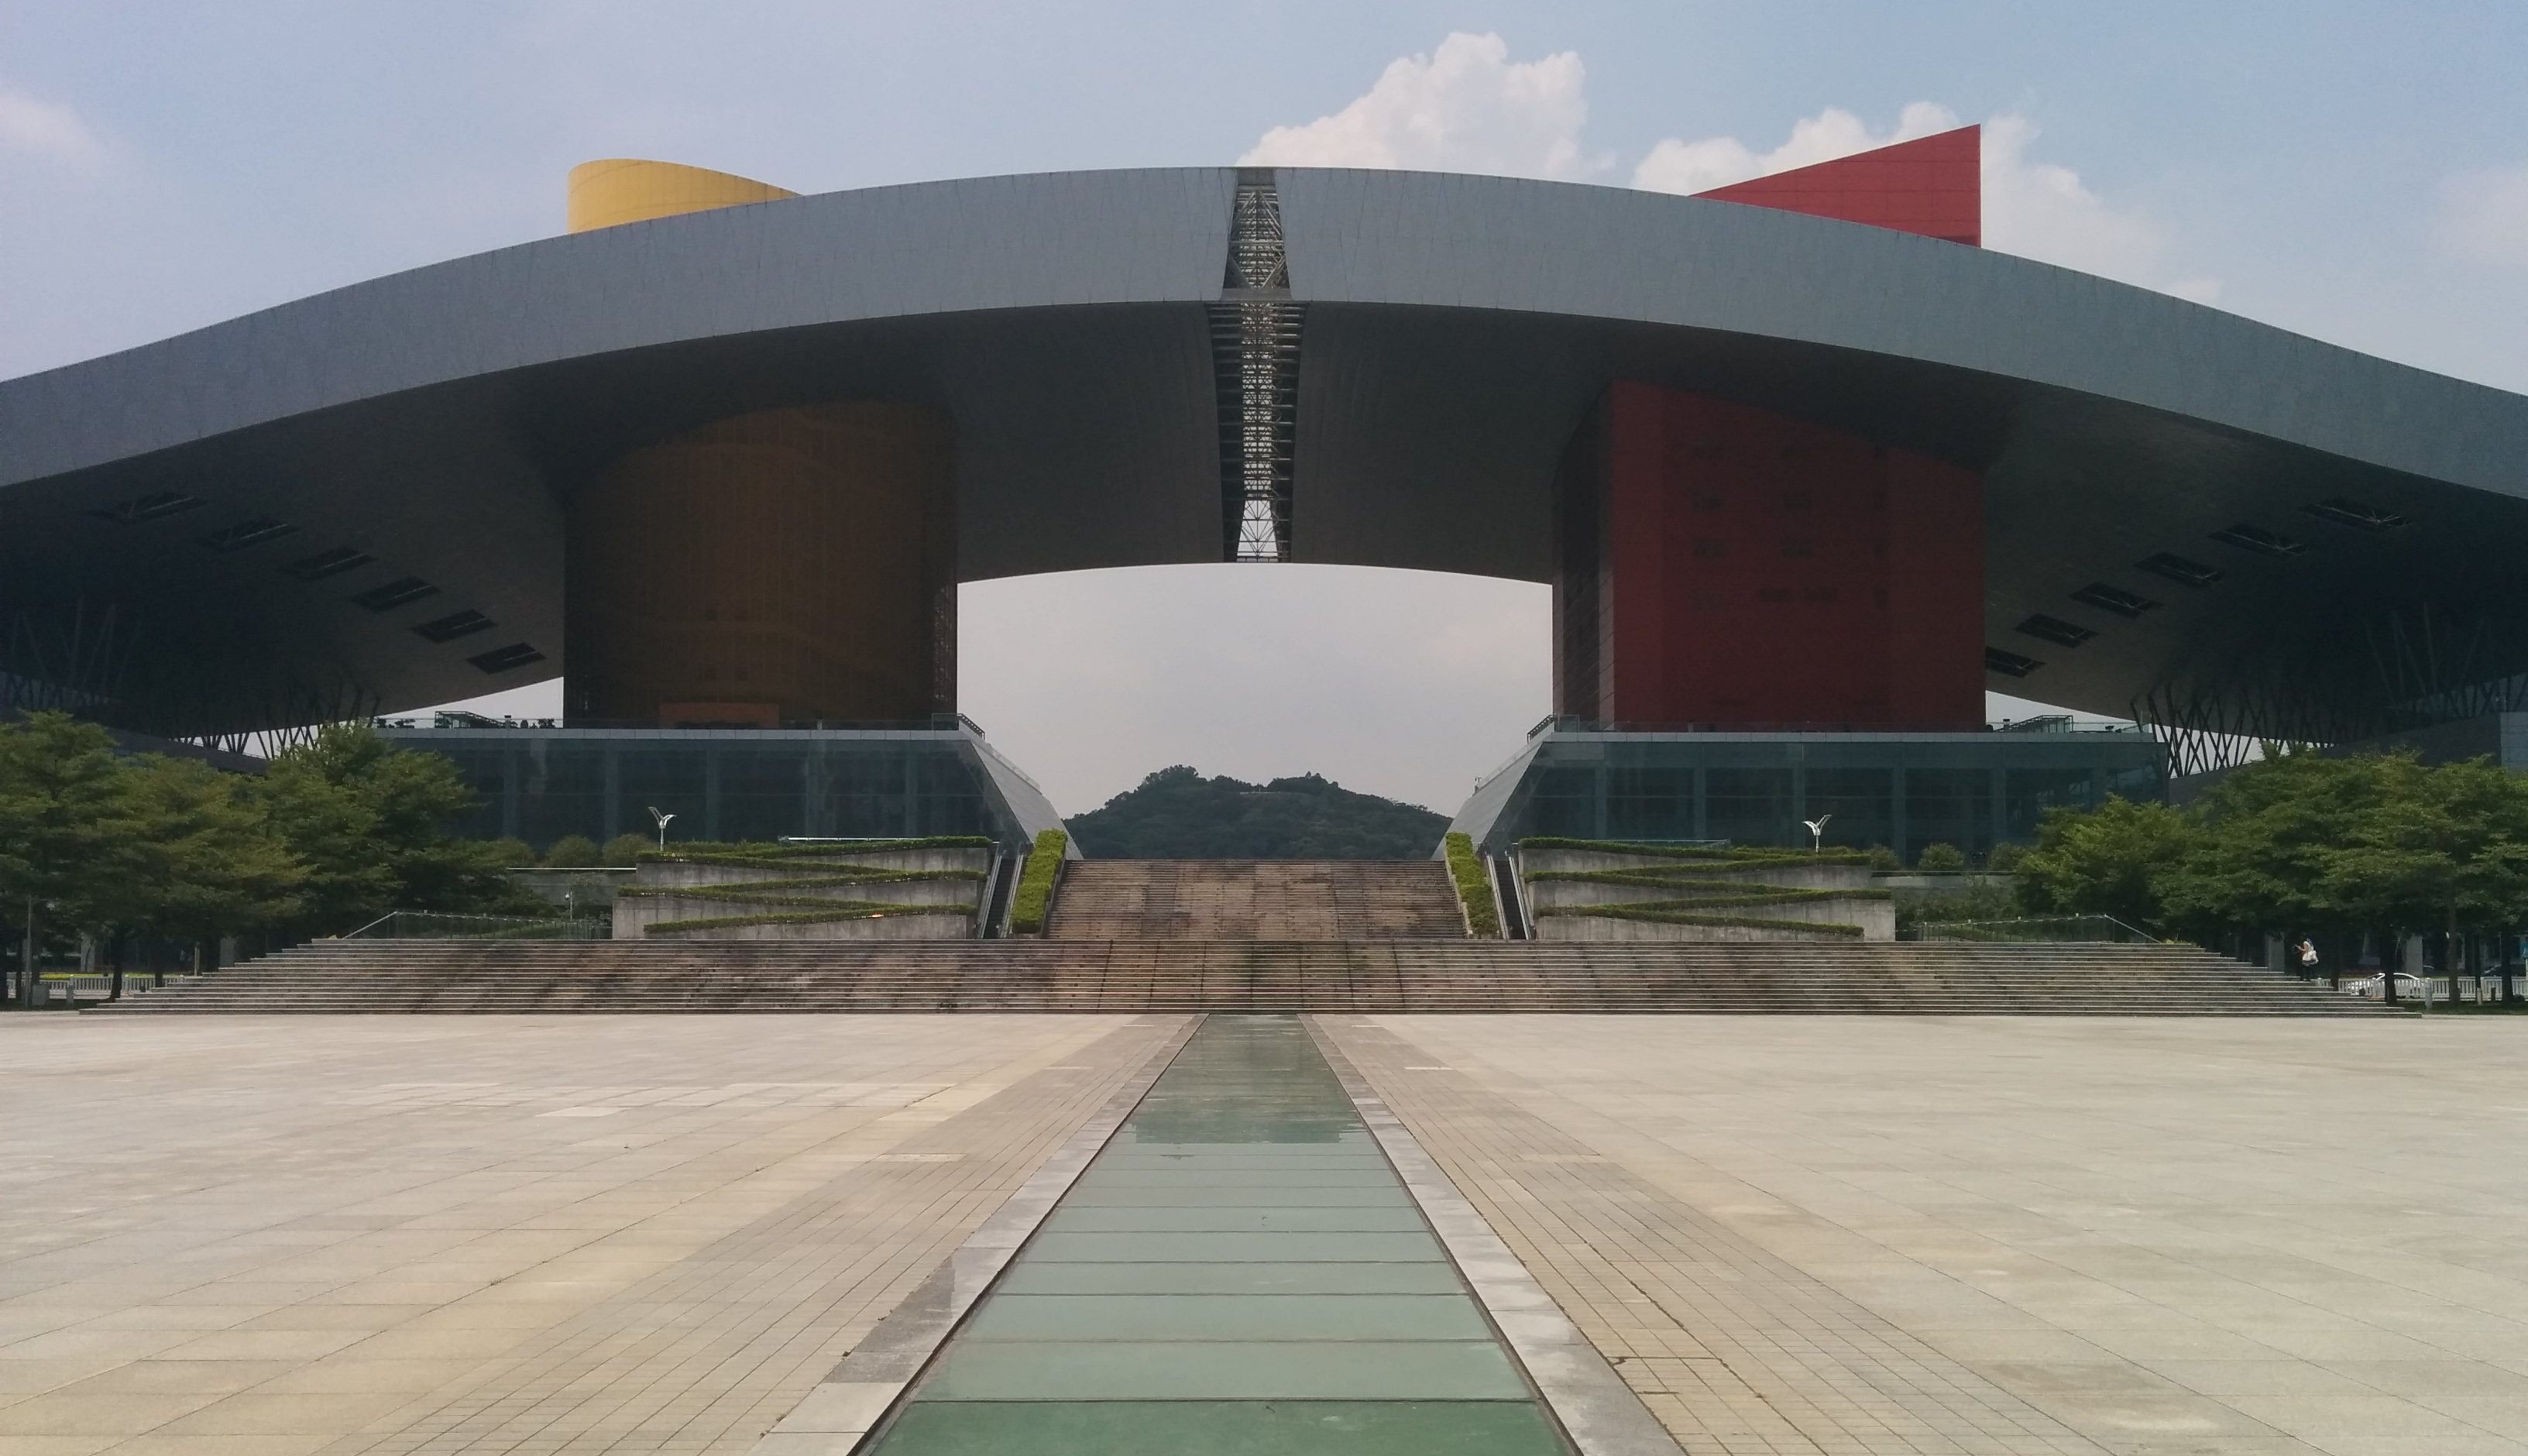
\includegraphics[width=\paperwidth]{img/shenzhen_convention_center.jpg}
	}
	\caption{Convention Center Shenzhen}
	\label{convention_center}
\end{figure}

Unter anderem hatten wir ein sehr interessantes Gespräch mit Vertretern
von \href{http://www.rolanddg.com/}{\emph{Roland}} über ein Kombigerät,
das sowohl schneiden als auch drucken kann. Das wäre für uns
interessant, da es womöglich einen größeren Funktionsumfang bei
ähnlichem Platzverbrauch bietet, als unser aktueller Schneideplotter.
Auch hatten wir Kontakt mit der österreichischen Firma
\href{https://www.troteclaser.com/}{\emph{Trotec}}. Schon seit längerem
interessiert sich das FAU FabLab für einen ihrer Lasercutter. So hatten
wir nun die Möglichkeit, einige Fragen zu klären und uns das Gerät
vorführen zu lassen. Sehr inspirierend war die Idee des chinesischen
Startups \href{http://dobot.cc/}{\emph{Dobot}}, die Funktionalitäten der
vielen Maschinen eines Labs in einem Multifunktionsroboterarm zu
Vereinen. So konnten wir beobachten, wie dieser 3D druckte und mit Laser
schneidete. Ein besonderes Feature dabei sind die APIs, womit es möglich
ist, eigene Anwendungen mit dem Roboter umzusetzen. Aus
sicherheitstechnischer Sicht kann man allerdings so ein Gerät nur schwer
in einem europäischen FabLab betreiben. Die Ausstellung des
\href{https://formlabs.com/}{\emph{FormLabs 2}} war mitunter der
Auslöser, unseren Wunsch und den Wunsch der Besucher, auf die Liste der
Studienzuschussanträge zu setzen. Wir liesen uns überzeugen, dass viele
Probleme, die noch bei der 1. Version des SLA Druckers bestanden, nun
behoben sind und er auch für unser FabLab eine Bereicherung ist.

Am Abend nahmen wir dann am Highlight der Konferenz Teil: Die
Auszeichnung der Teilnehmer an der
\href{http://fabacademy.org/}{FabAcademy}. In der FabAcademy werden
online gestreamte Vorlesungen mit Übungen in einem FabLab vor Ort
kombiniert. In Deutschland gibt es aktuell auf Grund der unzureichenden
Ausstattung kein FabLab das daran teilnimmt und anbietet Projekte dort
umzusetzen. Ein Deutscher Teilnehmer der FabAcademy absolviete seine
Übungsprojekte daher im FabLab Barcelona

Am \textbf{Samstag} durften wir noch in einer kleineren Runde eine Tour
durch Shenzhen machen. Die 1. Station war das
\href{https://www.fablabs.io/fablaboshenzhen}{FabLab O - Shenzen}, ein
FabLab das Designern und Künstlern einen großen Raum bot. Das FabLab ist
Teil einer Außestelle der Design Fakultät der Universität Tongji
(Shanghai). Die 2. Station war ein Startup Büro. Sie stellten uns ihr
aktuelles Projekt vor: ein Elektroroller für die Stadt. Die
Räumlichlkeiten, das Konzept und die Ausstattung waren sehr ähnlich, wie
das der bekannten FabLabs. Als letztes ging es dann noch zur Firma
Kunki. Diese fertigen Spritzgussteile für u.A. Mobiltelefone und
Automobile, allerdings mit Maschinen, die die Dimensionen von FabLabs
bei weitem übersteigen.

\section*{Workshops}

Neben den Talks und Vorträgen, bei denen es hauptsächlich um die
Entwicklung und Vernetzung der FabLabs in der Zukunft ging, wurden über
100 Workshops angeboten. Viele der Workshops können so oder in einer
abgewandelten Weise auch in unserem Fablab umgesetzt werden.

\subsection*{Färben von Stoffen mithilfe von Bakterien}

In diesem Workshop wurden Stoffe, in unserem Fall ein Schal, mithilfe
von Bakterien gefärbt. Da das Ziel eine Färbung im Batik Stil ist und
die Bakterien Luftsauerstoff benötigen, wurden im ersten Schritt die
Stoffstücke auf beliebige Art gefaltet, vernäht und zusammengebunden.
Hierdurch entsteht nur eine Färbung an der Oberfläche und ein
entsprechendes Muster. Anschließend wurden alle Utensilien, der Stoff
und die Nährlösung mithilfe eines Schnellkochtopfes sterilisiert. Im
letzten Schritt wurden die Stoffstücke mit einer Nährlösung getränkt und
mit einigen Bakterien bestrichen. Hierbei ist auf höchste Sauberkeit zu
achten, da die Bakterien sehr empfindlich sind und von vielen auf der
Haut oder in der Umgebung befindlichen Bakterien verdrängt werden.

\begin{figure}[htbp]
	\noindent\makebox[\textwidth]{
		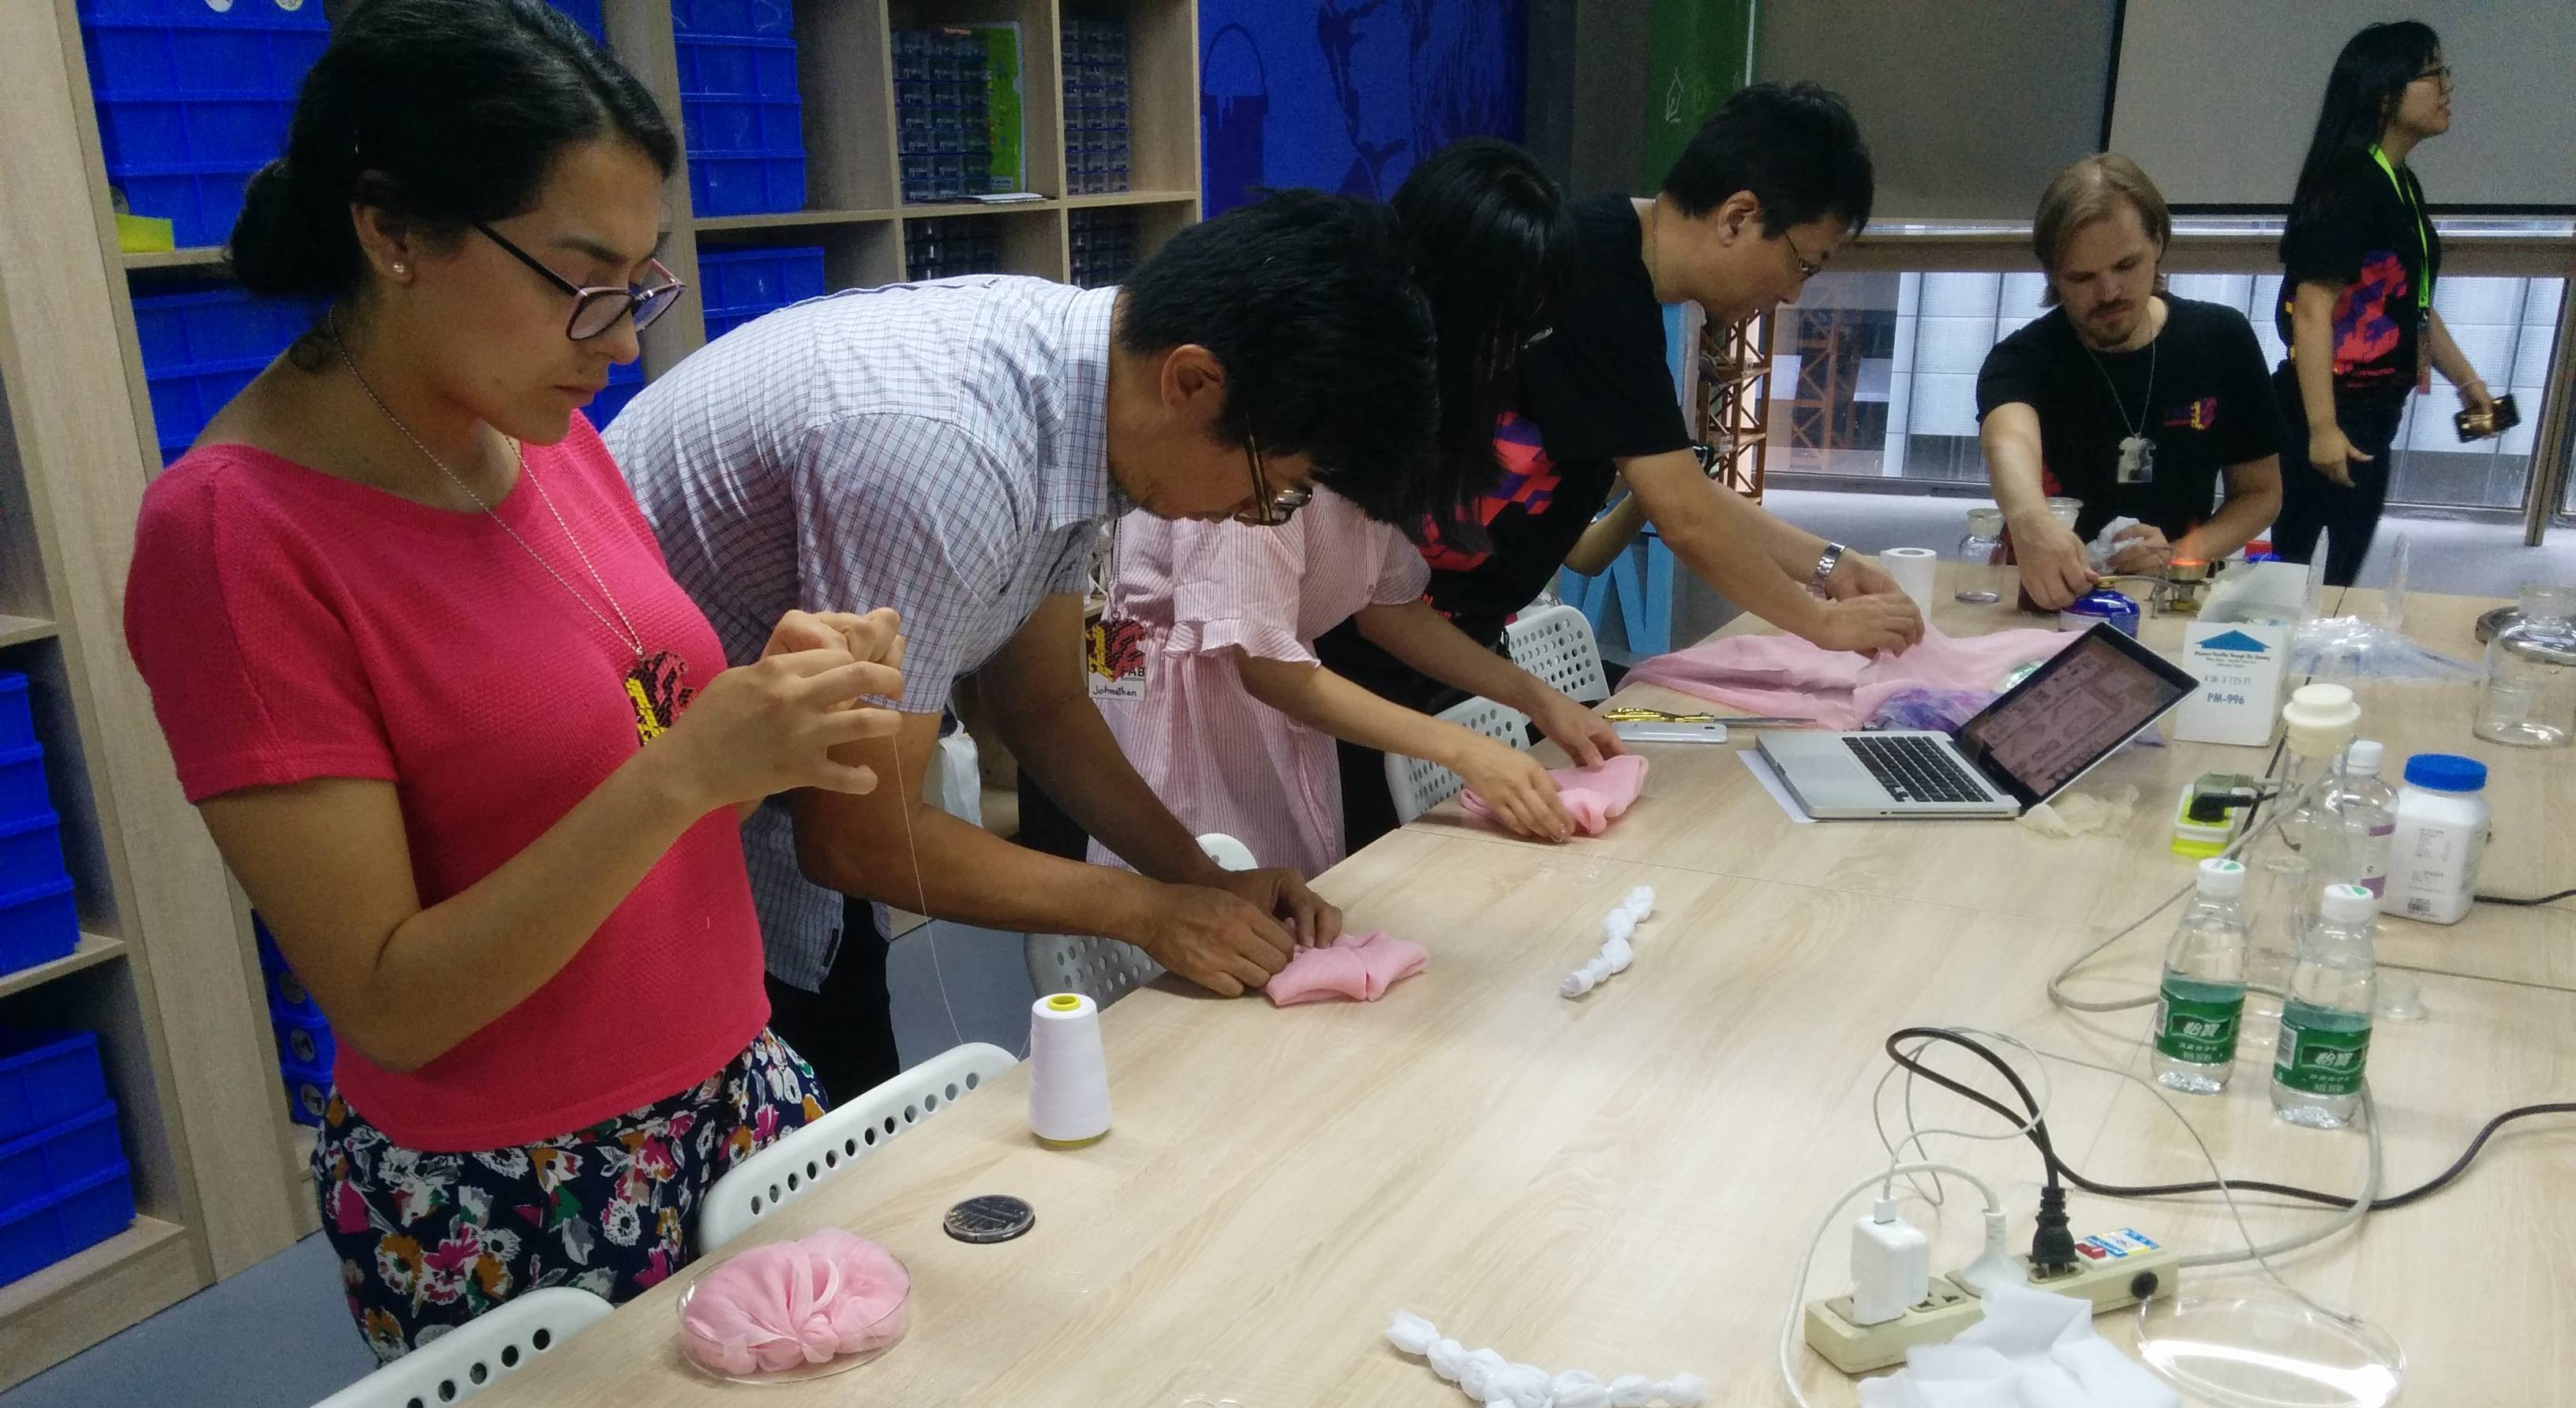
\includegraphics[width=\paperwidth]{img/bakterien.jpg}
	}
	\caption{Färben mit Bakterien}
	\label{faerben-von-stoffen-mithilfe-von-bakterien}
\end{figure}

\subsection*{SEEED Studio - From Prototyping to Manufacturing}

Bei SEEED Studio konnten wir den kompletten Weg von Entwicklung,
Prototypenfertigung bis hin zur ``Massenproduktion'' kennenlernen. Da
nur 3 Stunden für den Workshop angesetzt waren, musste natürlich etwas
einfacheres als eine Platine dafür herhalten. Wir sollten aus
vorhandenem Material innerhalb von 30 Minuten einen Schuh Prototyp
herstellen und ihn anschließend innerhalb von einer Stude so oft wie
möglich fertigen. Die auftretenden Probleme sind jedoch genau die selben
wie bei jedem anderen Produkt. In fast jeder Gruppe musste das Design
über den Workshop hinweg mehrmals geändert werden, unter anderem ging
das Material aus, das Design erforderte zu viel Nacharbeit oder die
Produktion war einfach zu kompliziert bzw. dauerte zu lange.

\subsection*{Bio Academy}

Ein Vertreter der Fab Foundation (Jean-Michel Molenar) stellte uns in
einem Vortrag das Prinzip der ``Bio Academy'' vor. Hierbei lernen
Beteiligte zunächst die Gefahren und Grenzen der Gentechnik kennen um
anschliessend selbst unter dem Motto ``How to Grow (almost) Anything''
Hand anlegen zu können. Es handelt sich hierbei um eine Art
Ringvorlesung, bei der verschiedene Dozenten Vorträge zu verschienenen
Themen halten. Anschliessend können die Teilnehmer analog zum
Übungsbetrieb an der Universität in einem Fablab praktische Erfahrungen
sammeln.

\subsection*{Game of Drones}

Zu Beginn erklärte Jonathan Doctorick wie er in fünftägigen Workshops
mit den Teilnehmern Miniatur Quadcopter baut. Diese Workshops führt er
mit seinem mobilen FabLab unter anderem mit Schülergruppen durch. Bei
diesen Workshops kann, neben Grundkenntnissen der Vektorbearbeitung,
auch der der Umgang mit einem Lötkolben zur Vervollständigung der
Elektronik näher gebracht werden. Die Motivation für Workshopteilnehmer
wird durch das abschließende Absolvieren einer Hindernisbahn gesteigert.
Im Anschluss an die Präsentation konnten wir in Gruppen einen eigenen
Quadcopterframe entwerfen und mit einem Lasercuter herstellen. Eine
Umsetzung eines ähnlichen Workshops in unserem FabLab würde
wahrscheinlich eine zweitägigen Workshop erfordern.

\subsection*{Build your own Fab-friendly experimental robot with multipurpose laser cut modules}

Dieser Workshop wurde von Mads Hobye von der Roskilde Universität
gehalten. Er selbst ist Dozent an dieser und führt diesen Workshop mit
Schülern, Studenten und teilweise auch Personal durch. Je nach
Zielgruppe werden hierbei aus vorhanden Bausätzen kleine Roboter gebaut
oder alternativ ein Programm entwickelt um entsprechende Bausätze zu
generieren. Da auch in diesem Workshop die Zeit begrenzt war, haben wir
uns auf den Bau eines kleinen Roboters aus den vorhanden Templates
beschränkt. Nach circa 2 Stunden und einer ordentlichen Portion
Heißkleber kam ein im kreis fahrender Putzroboter heraus.

Weitere informationen unter: \url{http://fablab.ruc.dk/construct/}

\begin{figure}[h]
	\noindent\makebox[\textwidth]{
		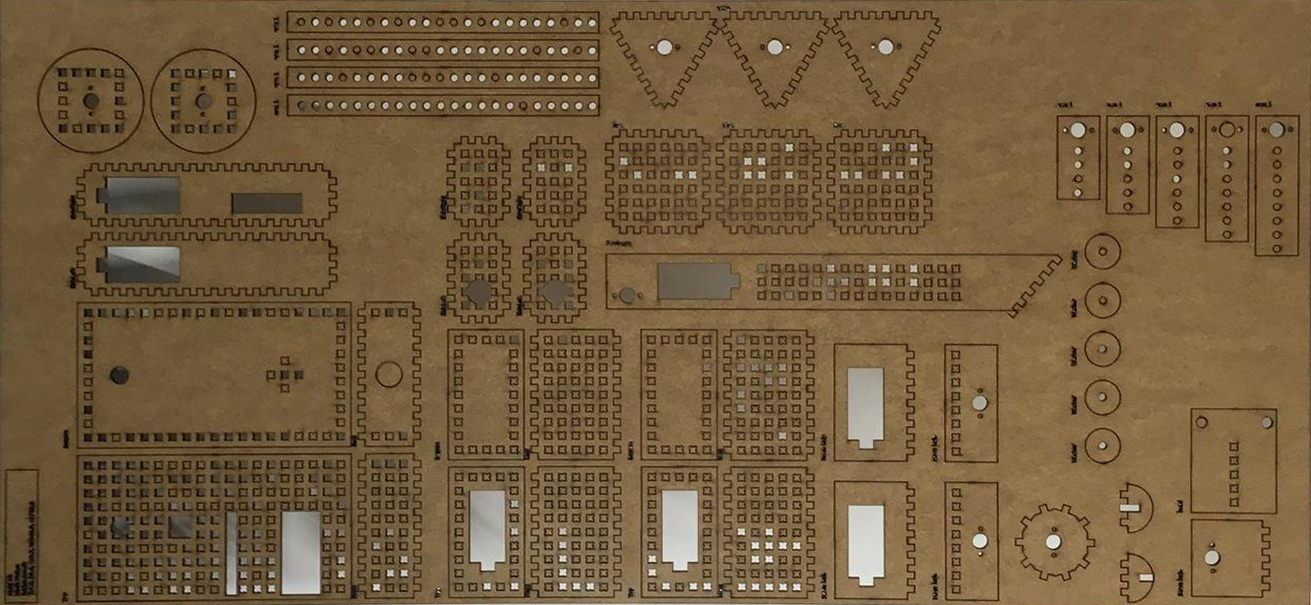
\includegraphics[width=\paperwidth]{img/roboter_bausatz.jpg}
	}
	\caption{Roboter Lasercut Template}
	\label{roboterbausatz}
\end{figure}
\begin{figure}[h]
	\noindent\makebox[\textwidth]{
		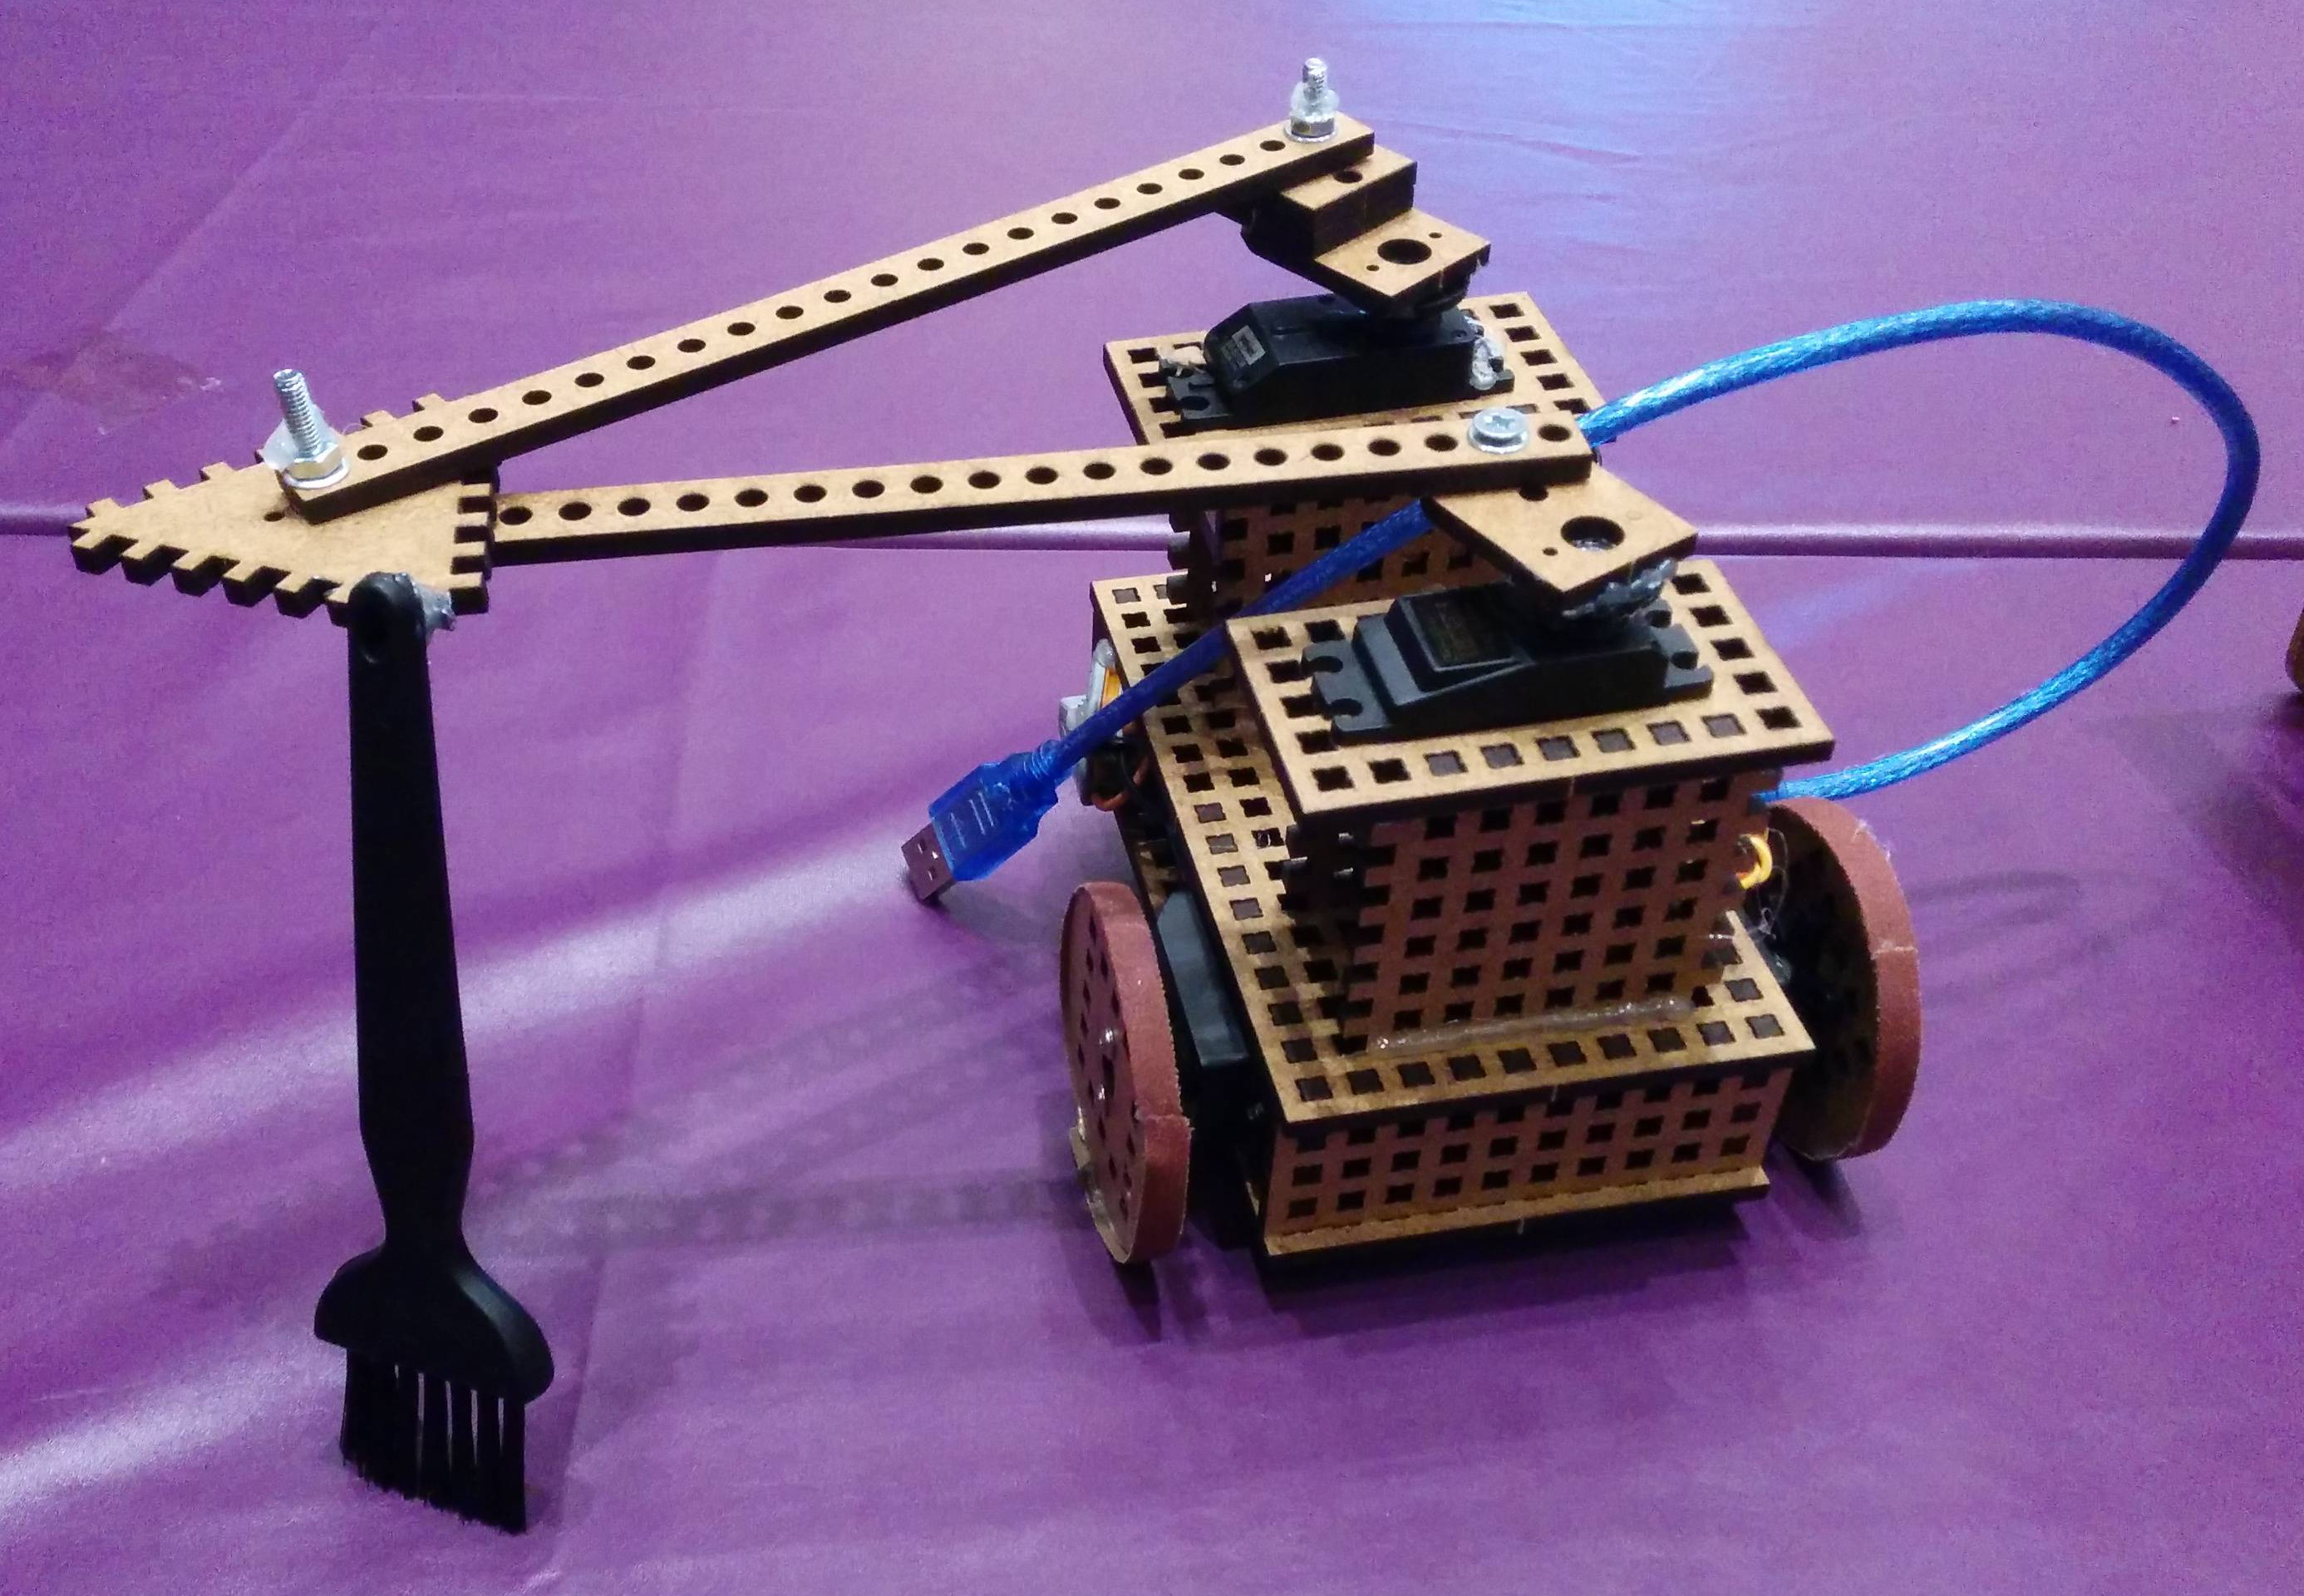
\includegraphics[width=\paperwidth]{img/selbstbau_roboter.jpg}
	}
	\caption{``Putzroboter''}
	\label{putzroboter}
\end{figure}

\subsection*{Make your own foldscope}

Jim Cybulski stellte das \href{https://en.wikipedia.org/wiki/Foldscope}{foldoscope}
vor - ein Mikroskop das auf
möglichst geringe Herstellungskosten optimiert ist. Es kann aus einem
Bogen Papier und einer Linse durch Falten ``hergestellt'' werden. Die
Teilnehmer bekamen einen Prototypen zum selbst ``zusammenbauen'' und
konnten anschliessend selbst diverse Gegenstände vergrößert betrachten,
was angesichts des geringen Herstellungsaufwands erstaunlich gut
funktionierte.

\subsection*{Making MIDI Musical Instrument, MMMI}

Uns wurde eine Plattform zum Herstellen von MIDI-Instrumenten
vorgestellt. Hierbei erhielten die Teilnehmer eine fertige
programmierbare Platine, an die sie eigene kapazitive Sensoren und
selbst gefertigte Gehäuse anschliessen konnten. Hierbei waren die zur
Verfügung gestellten Lasercutter und Materialen sehr hilfreich. Am Ende
ging jeder mit einem individuellen Instrument nach Hause.

\subsection*{Making Fablabs smarter through sensors and cloud based analysis}

Wie wäre es, wenn das FabLab mitdenken würde? In Zeiten von Internet Of
Things (IoT) ist das möglich. Matthias Friessnig aus dem
\href{http://fablab.tugraz.at/}{FabLab Graz} demonstrierte live, wie man
Sensordaten eines Ultimakers -- wie auch wir einen im FabLab haben --
erfassen und auswerten kann. Daten, wie z.B. die aktuelle Extruder
Temperatur, die Raumtemperatur, der Druckfortschrit oder der
Stromverbrauch lassen sich seiner Meinung nach unter anderem zur
Verbesserung der Produktion aber auch zum Abbrechen im Fehlerfall
verwenden. Ganz nach dem Prinzip ``Big Data'' versucht er in seinem
FabLab möglichst viele Maschinendaten zu erfassen und danach in der
Cloud auszuwerten. Nach einiger Zeit lassen sich sinnvolle Schlüsse
daraus ziehen. Leider ist dieser Schritt sehr aufwendig und es erfordert
viel Arbeit, bis aus dem Datensalat verwertbare Erkenntnisse entstehen.

\begin{figure}[htbp]
	\noindent\makebox[\textwidth]{
		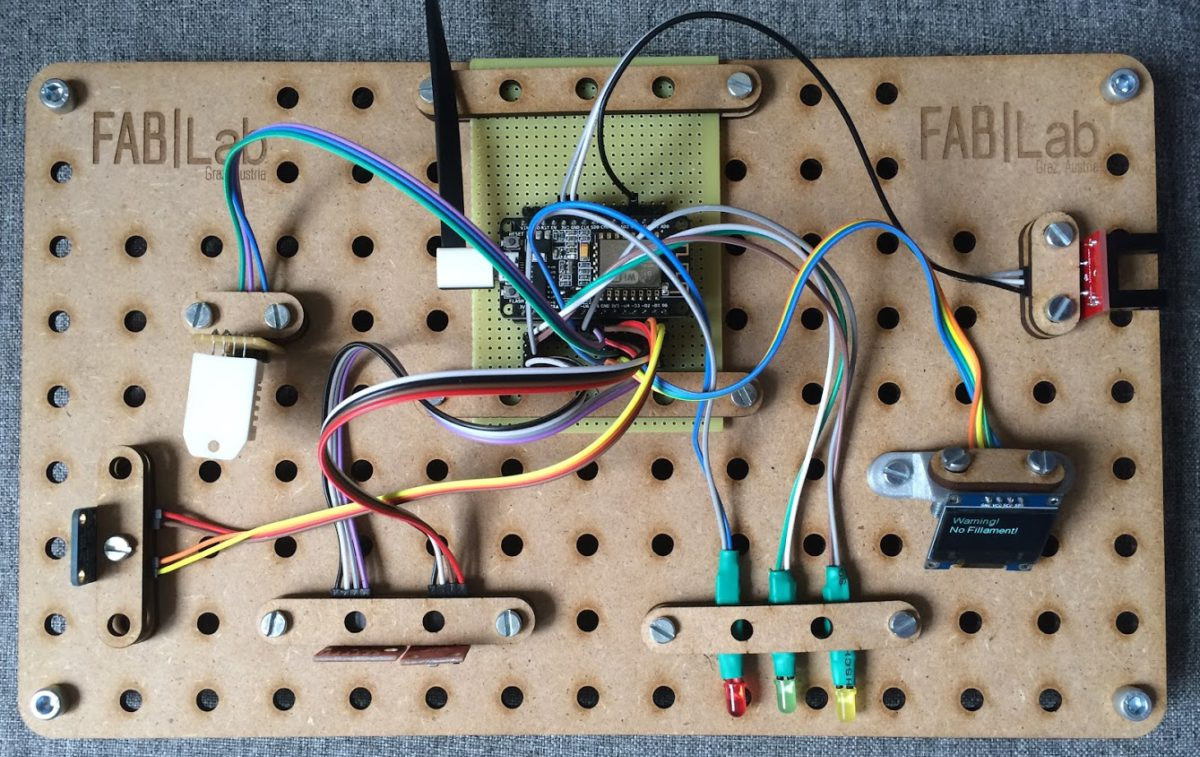
\includegraphics[width=\paperwidth]{img/sensors.jpg}
	}
	\caption{Portfolio von Matthias Friessnig:\\
	\url{http://fablab.tugraz.at/portfolio-item/making-fablabs-smarter-through-sensors-and-cloud-based-analysis/}}
	\label{sensors}
\end{figure}

\subsection*{Super-fun Design Hack}\label{super-fun-design-hack}

In einem etwas verrückten Workshop zeigten Ohad Meyuhas und Wendy Neale,
wie Designer und Künstler FabLabs verwenden können. Sie präsentierten
uns einen Hut, der aus nur einem Tonpapier gelasert wurde. Sie forderten
uns auf, die Vorlage zu ``hacken'' und etwas anderes auf die gleiche Art
durch Veränderung der Vorlage zu basteln. Es war sehr interessant zu
sehen, dass man nicht viel Vorwissen dazu braucht, sondern dass alleine
mit Kreativität auch schon viel möglich ist. Abschließend wurde
vorgeführt wie die am Anfang zur Verfügung gestellte Vorlage mit Hilfe
einer Parametrischen CAD Software hergestellt wurde.

\subsection*{Drawing CNC code}\label{drawing-cnc-code}

Im ersten Teil des Workshops versuchten wir in eine Art Würfel mit 3
Seiten einen Quader zu zeichnen, sodass er aus dieser aus einem
bestimmten Blickwinkel dreidimensional ausschaut. Dies ist uns auch mehr
oder weniger gelungen, aber es war gar nicht so einfach. Im zweiten Teil
erklärte uns Roberto Gallo, wie er dieses Prinzip verwendete um einen
Stift zu bauen, mit dem es möglich ist, GCode zu zeichnen. Dies war
seine Abschlussarbeit bei der FabAcademy.

Projekt von Roberto Gallo bei der FabAcademy 2016:\\ \url{http://archive.fabacademy.org/archives/2016/fablabyachay/students/302/fproject.html}

\section*{Fazit}\label{fazit}

Es war großartig als eines von über 450 FabLabs an dem
Event teilzunehmen und diese internationale Athmosphäre zu erleben. Wir
hatten so die Chance die weltweite FabLabbewegung kennen zu lernen und
können jetzt unser FabLab besser in die globale Struktur einordnen.
Allen beteiligten Departments möchten wir sehr herzlich danken, dass sie
uns diese Bereicherung möglich gemacht haben.

\vspace{1cm}
\LARGE
\centering
\begin{CJK}{UTF8}{gbsn}
	谢谢\\
	xi\`exie
\end{CJK}
	
\end{document}
